\documentclass[aspectratio=169]{beamer}

% ---------- Theme & Navigation ----------
\usetheme{default}
\setbeamertemplate{navigation symbols}{}
\setbeamertemplate{footline}{}

\usepackage[T1]{fontenc}
\usepackage[utf8]{inputenc}
\usepackage{lmodern}
\usepackage{booktabs}
\usepackage{array}
\usepackage{graphicx}
\usepackage{tikz}
\usepackage{fontawesome5}
\usepackage{calc}
\usetikzlibrary{arrows.meta,positioning,shapes.geometric,calc,decorations.pathmorphing,backgrounds,fit,shadows}
\usepackage{colortbl}

% ---------- Color Palette (Deep Teal + Warm Coral) ----------
\definecolor{DarkBg}{RGB}{18,25,38}
\definecolor{DeepTeal}{RGB}{0,128,128}
\definecolor{LightTeal}{RGB}{0,180,170}
\definecolor{Coral}{RGB}{255,107,107}
\definecolor{SoftCoral}{RGB}{255,150,130}
\definecolor{Gold}{RGB}{255,193,37}
\definecolor{Cream}{RGB}{250,248,244}
\definecolor{LightGray}{RGB}{240,243,247}
\definecolor{MidGray}{RGB}{120,130,150}
\definecolor{DarkText}{RGB}{30,40,55}
\definecolor{AccentPurple}{RGB}{130,100,220}
\definecolor{GradStart}{RGB}{0,100,110}
\definecolor{GradEnd}{RGB}{0,155,145}
\definecolor{CardBg}{RGB}{255,255,255}
\definecolor{CardBorder}{RGB}{220,225,235}

% ---------- Beamer Colors ----------
\setbeamercolor{normal text}{fg=DarkText}
\setbeamercolor{structure}{fg=DeepTeal}
\setbeamercolor{frametitle}{fg=white}
\setbeamercolor{title}{fg=white}
\setbeamercolor{subtitle}{fg=Cream}
\setbeamercolor{author}{fg=Cream}
\setbeamercolor{institute}{fg=LightTeal}
\setbeamercolor{date}{fg=Gold}
\setbeamercolor{block title}{bg=DeepTeal,fg=white}
\setbeamercolor{block body}{bg=LightGray,fg=DarkText}
\setbeamercolor{itemize item}{fg=DeepTeal}
\setbeamercolor{itemize subitem}{fg=Coral}
\setbeamercolor{enumerate item}{fg=DeepTeal}

% ---------- Beamer Fonts ----------
\setbeamerfont{title}{size=\Large,series=\bfseries}
\setbeamerfont{subtitle}{size=\normalsize}
\setbeamerfont{frametitle}{size=\large,series=\bfseries}
\setbeamerfont{block title}{size=\normalsize,series=\bfseries}

% ---------- Itemize Style ----------
\setbeamertemplate{itemize item}{\scriptsize\raise1.5pt\hbox{\textcolor{DeepTeal}{\rule{5pt}{5pt}}}}
\setbeamertemplate{itemize subitem}{\scriptsize\raise1.5pt\hbox{\textcolor{Coral}{$\blacktriangleright$}}}
\setbeamertemplate{enumerate item}{\insertenumlabel.}

% ---------- Frame Title Bar ----------
\setbeamertemplate{frametitle}{%
  \nointerlineskip
  \begin{beamercolorbox}[wd=\paperwidth,ht=1.1cm,dp=0.2cm,leftskip=0.8cm,rightskip=0.3cm]{frametitle}
    \tikz[remember picture,overlay]{
      \fill[left color=GradStart,right color=GradEnd] (-0.8cm,-0.2cm) rectangle (\paperwidth,1.1cm);
      \fill[Coral] (-0.8cm,-0.2cm) rectangle (\paperwidth,-0.14cm);
    }
    \strut\insertframetitle\strut
  \end{beamercolorbox}
}

% ---------- Slide Number (bottom-right, subtle) ----------
\addtobeamertemplate{footline}{}{%
  \hfill\usebeamercolor[fg]{normal text}{\scriptsize\color{MidGray}\insertframenumber\kern1.5em\vskip1em}%
}

% ---------- Background Decoration ----------
\setbeamertemplate{background}{%
  
\begin{tikzpicture}[remember picture,overlay]
    % Subtle corner accent
    \fill[DeepTeal,opacity=0.04] (current page.south west) -- ++(3,0) -- ++(0,3) -- cycle;
    \fill[Coral,opacity=0.03] (current page.north east) -- ++(-2.5,0) -- ++(0,-2.5) -- cycle;
  \end{tikzpicture}
}

% ---------- Custom Commands ----------
\newcommand{\callout}[1]{%
  \vspace{0.5em}%
  \begin{tikzpicture}
    \node[fill=Gold!12,draw=Gold!50,rounded corners=4pt,inner sep=8pt,text width=\linewidth-24pt,font=\small] {%
      \textcolor{Gold!80!black}{\faIcon{lightbulb}}\;\textcolor{DarkText}{#1}};
  \end{tikzpicture}%
}
\newcommand{\metric}[2]{\textbf{#1}: #2}

% Card-style block
\newcommand{\card}[2]{%
  \begin{tikzpicture}
    \node[fill=CardBg,draw=CardBorder,rounded corners=5pt,inner sep=9pt,text width=\linewidth-26pt,drop shadow={shadow xshift=0.5pt,shadow yshift=-0.5pt,fill=black!8}] {%
      {\bfseries\color{DeepTeal}#1}\par\smallskip #2};
  \end{tikzpicture}%
}

% Icon bullet
\newcommand{\iconitem}[2]{\item[\textcolor{DeepTeal}{\faIcon{#1}}] #2}

% ---------- Title Page ----------
\title{Distributed Energy Monitoring Platform}
\subtitle{Distributed Systems Course Project}
\author{Youness Anouar - Mouad El Ansari - Jaafar Yeffou}
\institute{UM6P College Of Computing}
\date{April 7, 2026}

\setbeamertemplate{title page}{%
  \begin{tikzpicture}[remember picture,overlay]
    % Full-slide dark gradient background
    \fill[left color=DarkBg,right color=DarkBg!85!DeepTeal] (current page.south west) rectangle (current page.north east);
    % Decorative mesh circles
    \fill[LightTeal,opacity=0.06] ([shift={(2cm,2cm)}]current page.south west) circle (2.5cm);
    \fill[LightTeal,opacity=0.05] ([shift={(-2cm,2cm)}]current page.south east) circle (3cm);
    \fill[LightTeal,opacity=0.07] ([shift={(-3cm,-1.5cm)}]current page.north east) circle (1.8cm);
    \fill[LightTeal,opacity=0.04] ([shift={(4cm,1cm)}]current page.south west) circle (1.5cm);
    % Accent line at bottom
    \fill[Coral] ([yshift=0.7cm]current page.south west) rectangle ([yshift=0.76cm]current page.south east);
    \fill[Gold,opacity=0.7] ([yshift=0.62cm]current page.south west) rectangle ([yshift=0.68cm]current page.south east);
    % ---- Centered text block ----
    % A thin decorative rule above the title
    \fill[LightTeal,opacity=0.6]
      ([shift={(-4cm,2.6cm)}]current page.center) rectangle ([shift={(4cm,2.64cm)}]current page.center);
    % Title
    \node[text width=12cm,align=center] at ([yshift=1.7cm]current page.center) {%
      {\fontsize{24}{30}\selectfont\bfseries\color{white}\inserttitle}};
    % Subtitle
    \node[text width=12cm,align=center] at ([yshift=0.5cm]current page.center) {%
      {\large\color{LightTeal}\insertsubtitle}};
    % A thin decorative rule below the subtitle
    \fill[LightTeal,opacity=0.6]
      ([shift={(-3cm,-0.1cm)}]current page.center) rectangle ([shift={(3cm,-0.06cm)}]current page.center);
    % Author
    \node[text width=12cm,align=center] at ([yshift=-0.8cm]current page.center) {%
      {\normalsize\color{Cream}\insertauthor}};
    % Institute | Date
    \node[text width=12cm,align=center] at ([yshift=-1.4cm]current page.center) {%
      {\small\color{MidGray}\insertinstitute\quad\textcolor{Gold}{|}\quad\insertdate}};
    % ---- Decorative icons (right side, faded) ----
    \node[font=\fontsize{44}{44}\selectfont,text=DeepTeal,opacity=0.18]
      at ([shift={(5cm,2cm)}]current page.center) {\faIcon{bolt}};
    \node[font=\fontsize{30}{30}\selectfont,text=Coral,opacity=0.14]
      at ([shift={(6.2cm,0.2cm)}]current page.center) {\faIcon{server}};
    \node[font=\fontsize{26}{26}\selectfont,text=Gold,opacity=0.14]
      at ([shift={(4.2cm,-0.5cm)}]current page.center) {\faIcon{chart-line}};
    % Mirror a faint icon on the left for balance
    \node[font=\fontsize{30}{30}\selectfont,text=LightTeal,opacity=0.10]
      at ([shift={(-5.5cm,1.8cm)}]current page.center) {\faIcon{microchip}};
    \node[font=\fontsize{24}{24}\selectfont,text=MidGray,opacity=0.10]
      at ([shift={(-6cm,-0.3cm)}]current page.center) {\faIcon{network-wired}};
  \end{tikzpicture}
}

\begin{document}

% ==================== SLIDE 1: TITLE ====================
\begin{frame}[plain]
  \titlepage
\end{frame}

% ==================== SLIDE 2: THE CHALLENGE ====================
\begin{frame}{The Challenge}
  \begin{columns}[T]
    \column{0.54\textwidth}
      \card{The Problem}{%
        \small Labs and organizations operate many workstations, servers, and Raspberry Pis, but energy usage is \textbf{fragmented} and often \textbf{invisible} in real time.}
      \vspace{0.3em}
      \begin{itemize}\setlength\itemsep{0.1em}
        \iconitem{eye-slash}{No unified view of live power consumption}
        \iconitem{database}{No historical data for optimization}
        \iconitem{unlink}{Local-only monitoring creates data silos}
        \iconitem{clock}{Manual sampling is too slow for operations}
      \end{itemize}
    \column{0.42\textwidth}
      \centering
      \begin{tikzpicture}[
        box/.style={draw=DeepTeal!70, rounded corners=4pt, thick, fill=white, minimum width=2.5cm, minimum height=0.8cm, align=center, font=\small, drop shadow={shadow xshift=0.3pt,shadow yshift=-0.3pt,fill=black!6}},
        q/.style={font=\Large\bfseries\color{Coral}}
      ]
        \node[box] (n1) at (0,2.0) {\faIcon{desktop}\; Workstation};
        \node[box] (n2) at (0,0.9) {\faIcon{server}\; Server};
        \node[box] (n3) at (0,-0.2) {\faIcon{microchip}\; Raspberry Pi};
        \node[q] at (2.2,2.0) {\faIcon{question-circle}};
        \node[q] at (2.2,0.9) {\faIcon{question-circle}};
        \node[q] at (2.2,-0.2) {\faIcon{question-circle}};
      \end{tikzpicture}
  \end{columns}

  \callout{Goal: build one distributed system that scales from 10 to 10,000 nodes without redesigning the API or database.}
\end{frame}

% ==================== SLIDE 3: KPIS ====================
\begin{frame}{What KPIs Do We Monitor?}
  \begin{columns}[T]
    \column{0.48\textwidth}
      \card{\faIcon{tachometer-alt}\; Node-Level KPIs}{%
        \begin{itemize}\setlength\itemsep{0.2em}
          \item \textbf{Power (W)}: real or estimated node consumption
          \item \textbf{CPU usage}: utilization per machine
          \item \textbf{Memory usage}: RAM pressure over time
          \item \textbf{Temperature}: thermal behavior when available
        \end{itemize}}
      \vspace{0.35em}
      \card{\faIcon{heartbeat}\; Health KPI}{%
        \textbf{Node status}: \textcolor{DeepTeal}{ONLINE} / \textcolor{Gold!80!black}{STALE} / \textcolor{Coral}{OFFLINE}}
    \column{0.48\textwidth}
      \card{\faIcon{layer-group}\; Application-Level KPIs}{%
        \begin{itemize}\setlength\itemsep{0.2em}
          \item \textbf{Per-app power}: who consumes the most energy
          \item \textbf{Per-app CPU share}: workload attribution
          \item \textbf{Top consumers}: ranking of active processes
        \end{itemize}}
      \vspace{0.35em}
      \card{\faIcon{chart-line}\; Why These KPIs Matter}{%
        \begin{itemize}\setlength\itemsep{0.2em}
          \item Detect overloaded or unhealthy nodes
          \item Identify power-hungry applications
          \item Compare live behavior with historical trends
        \end{itemize}}
  \end{columns}

  \callout{These KPIs turn raw measurements into operational signals for monitoring, optimization, and fault detection.}
\end{frame}

% ==================== SLIDE 3: WHY DISTRIBUTED ====================
\begin{frame}{Why This Is a Distributed Systems Problem}
  \begin{columns}[T]
    \column{0.55\textwidth}
      \begin{itemize}
        \iconitem{network-wired}{\textbf{Heterogeneous infrastructure}: Linux, Windows, and RPi expose different measurement interfaces.}
        \iconitem{wifi}{\textbf{Network unreliability}: nodes may disconnect unpredictably.}
        \iconitem{clock}{\textbf{Temporal consistency}: distributed sources send at different rates.}
        \iconitem{expand-arrows-alt}{\textbf{Scalability}: aggregate large metric volumes in near real time.}
        \iconitem{heartbeat}{\textbf{Fault detection}: distinguish network jitter from actual failure.}
      \end{itemize}
    \column{0.42\textwidth}
      \vspace{0.5em}
      \card{Design Philosophy}{%
        \begin{itemize}
          \item[\textcolor{DeepTeal}{\faIcon{cog}}] Autonomous daemons
          \item[\textcolor{DeepTeal}{\faIcon{sync}}] Eventual consistency
          \item[\textcolor{DeepTeal}{\faIcon{brain}}] Adaptive fault detection
          \item[\textcolor{DeepTeal}{\faIcon{database}}] Time-series storage
        \end{itemize}}
  \end{columns}
\end{frame}

% ==================== SLIDE 4: ARCHITECTURE ====================
\begin{frame}{Architecture at 10,000 Feet}
  \begin{columns}[c]
    \column{0.48\textwidth}
      \centering
      \begin{tikzpicture}[
        node distance=0.5cm,
        basebox/.style={rounded corners=4pt, thick, align=center, minimum width=3.8cm, minimum height=0.95cm, font=\scriptsize},
        arrow/.style={-{Latex[length=2.5mm]}, thick, draw=MidGray},
        lbl/.style={font=\tiny\color{MidGray},fill=white,inner sep=1.5pt}
      ]
        \node[basebox, draw=AccentPurple!70, fill=AccentPurple!8] (viz) {\faIcon{chart-area}\; \textbf{Visualization Layer}\\React Dashboard};
        \node[basebox, draw=Coral!70, fill=Coral!8, below=of viz] (api) {\faIcon{cogs}\; \textbf{Aggregation Layer}\\FastAPI Backend};
        \node[basebox, draw=DeepTeal!70, fill=DeepTeal!8, below=of api] (daemon) {\faIcon{robot}\; \textbf{Collection Layer}\\Python Daemons};
        \node[basebox, draw=Gold!70, fill=Gold!8, below=of daemon] (measure) {\faIcon{bolt}\; \textbf{Measurement Layer}\\RAPL / psutil / INA219};

        \draw[arrow] (measure) -- node[lbl,right]{hardware APIs} (daemon);
        \draw[arrow] (daemon) -- node[lbl,right]{HTTP POST} (api);
        \draw[arrow] (api) -- node[lbl,right]{REST API} (viz);
      \end{tikzpicture}
    \column{0.48\textwidth}
      \begin{itemize}\setlength\itemsep{0.4em}
        \iconitem{upload}{\textbf{Push architecture}: nodes send data proactively.}
        \iconitem{clone}{\textbf{Stateless backend}: easy horizontal replication.}
        \iconitem{database}{\textbf{ClickHouse}: fast real-time and historical queries.}
      \end{itemize}
  \end{columns}
\end{frame}

% ==================== SLIDE 5: DS PRINCIPLES ====================
\begin{frame}{Distributed Systems Principles Applied}
  \begin{columns}[T]
    \column{0.48\textwidth}
      \card{\faIcon{shield-alt}\; Fault Tolerance}{\small%
        \begin{itemize}\setlength\itemsep{0pt}
          \item File-backed retry buffer
          \item Exponential backoff
          \item Daemon collects while backend is down
        \end{itemize}}
      \vspace{0.25em}
      \card{\faIcon{sync}\; Eventual Consistency}{\small%
        \begin{itemize}\setlength\itemsep{0pt}
          \item Nodes send independently
          \item Out-of-order arrival is acceptable
          \item Storage reconciles time-series state
        \end{itemize}}
    \column{0.48\textwidth}
      \card{\faIcon{heartbeat}\; Adaptive Health Checking}{\small%
        \begin{itemize}\setlength\itemsep{0pt}
          \item Learned timeout per node
          \item ONLINE $\rightarrow$ STALE $\rightarrow$ OFFLINE
          \item 4$\sigma$ threshold for low false positives
        \end{itemize}}
      \vspace{0.25em}
      \card{\faIcon{expand-arrows-alt}\; Horizontal Scalability}{\small%
        \begin{itemize}\setlength\itemsep{0pt}
          \item Add nodes by deploying more daemons
          \item Add API replicas without coordination
          \item Same schema and query interface
        \end{itemize}}
  \end{columns}
\end{frame}

% ==================== SLIDE 6: HETEROGENEOUS COLLECTION ====================
\begin{frame}{Smart Solution 1: Heterogeneous Data Collection}
  \begin{columns}[T]
    \column{0.54\textwidth}
      \card{\faIcon{puzzle-piece}\; Unified Interface, Different Backends}{%
        \begin{itemize}
          \item \textbf{Linux}: Intel RAPL for direct hardware readings
          \item \textbf{Windows}: psutil-based estimation
          \item \textbf{Raspberry Pi}: INA219 sensor over I\textsuperscript{2}C
          \item \textbf{Fallback}: estimate from CPU when direct measurement is missing
        \end{itemize}}
      \vspace{0.3em}
      \callout{Adapter pattern keeps one daemon API while supporting multiple platforms.}
    \column{0.42\textwidth}
      \vspace{0.3em}
      \begin{table}
        \scriptsize
        \rowcolors{2}{LightGray}{white}
        \begin{tabular}{@{}lll@{}}
          \toprule
          \textbf{Platform} & \textbf{Method} & \textbf{Fidelity} \\
          \midrule
          Linux & RAPL & \textcolor{DeepTeal}{\faIcon{circle}\; High} \\
          Windows & CPU estimate & \textcolor{Gold}{\faIcon{circle}\; Medium} \\
          RPi & INA219 & \textcolor{DeepTeal}{\faIcon{circle}\; High} \\
          Generic & Fallback & \textcolor{Gold}{\faIcon{circle}\; Medium} \\
          \bottomrule
        \end{tabular}
      \end{table}
      \vspace{0.5em}
      \card{\faIcon{tags}\; Schema Tags}{%
        \texttt{\small node\_type}\\
        \texttt{\small measurement\_method}}
  \end{columns}
\end{frame}

% ==================== SLIDE 7: RELIABLE INGESTION ====================
\begin{frame}{Smart Solution 2: Reliable Ingestion}
  \begin{columns}[T]
    \column{0.52\textwidth}
      \card{\faIcon{redo}\; Retry Buffer}{%
        \begin{enumerate}
          \item Collect metrics every 5--10 seconds
          \item Persist locally first
          \item Try HTTP POST to backend
          \item On failure, keep data in local buffer
          \item Retry with exponential backoff
        \end{enumerate}}
      \vspace{0.3em}
      \callout{No data loss during temporary outages and no dependency on constant connectivity.}
    \column{0.44\textwidth}
      \centering
      \vspace{0.3em}
      \begin{tikzpicture}[
        smallbox/.style={draw=DeepTeal!60, rounded corners=3pt, fill=white, align=center, minimum width=1.9cm, minimum height=0.6cm, font=\tiny, drop shadow={shadow xshift=0.3pt,shadow yshift=-0.3pt,fill=black!6}},
        arrow/.style={-{Latex[length=2mm]}, thick, draw=DeepTeal!60},
        ok/.style={-{Latex[length=2mm]}, thick, draw=DeepTeal},
        fail/.style={-{Latex[length=2mm]}, thick, draw=Coral}
      ]
        \node[smallbox] (c1) {\faIcon{bolt}\; Collect metric};
        \node[smallbox, below=0.4cm of c1] (c2) {\faIcon{save}\; Write to buffer};
        \node[smallbox, below=0.4cm of c2] (c3) {\faIcon{paper-plane}\; Send to backend};
        \node[smallbox, fill=DeepTeal!6, below left=0.5cm and -0.1cm of c3] (c4) {\textcolor{DeepTeal}{\faIcon{check}}\; Remove};
        \node[smallbox, fill=Coral!6, below right=0.5cm and -0.1cm of c3] (c5) {\textcolor{Coral}{\faIcon{redo}}\; Retry};

        \draw[arrow] (c1) -- (c2);
        \draw[arrow] (c2) -- (c3);
        \draw[ok] (c3) -- (c4);
        \draw[fail] (c3) -- (c5);
      \end{tikzpicture}
  \end{columns}
\end{frame}

% ==================== SLIDE 8: HEARTBEAT DETECTION ====================
\begin{frame}{Smart Solution 3: Adaptive Heartbeat Detection}
  \begin{columns}[T]
    \column{0.56\textwidth}
      \card{\faIcon{brain}\; k-Sigma Timeout}{%
        \[
          \text{timeout} = \mu_{\text{interval}} + 4 \times \sigma_{\text{interval}}
        \]}
      \vspace{0.3em}
      \begin{itemize}
        \iconitem{tachometer-alt}{Fast nodes get short timeouts}
        \iconitem{hourglass-half}{Slow nodes get relaxed timeouts}
        \iconitem{adjust}{STALE state absorbs temporary jitter}
        \iconitem{exclamation-triangle}{OFFLINE declared only after stronger evidence}
      \end{itemize}
      \callout{Mimics heartbeat-based fault detection used in production distributed systems.}
    \column{0.4\textwidth}
      \vspace{0.3em}
      \begin{table}
        \scriptsize
        \rowcolors{2}{LightGray}{white}
        \begin{tabular}{@{}lll@{}}
          \toprule
          \textbf{Node} & \textbf{Pattern} & \textbf{Timeout} \\
          \midrule
          Node-1 & 10s, stable & 10.6s \\
          Node-2 & 60s, slower & 68s \\
          Node-3 & variable & 55s \\
          \bottomrule
        \end{tabular}
      \end{table}
      \vspace{0.5em}
      \card{\faIcon{traffic-light}\; Health States}{%
        \scriptsize
        \textcolor{DeepTeal}{\faIcon{circle}\; \textbf{ONLINE}}: age $<$ timeout\\
        \textcolor{Gold}{\faIcon{circle}\; \textbf{STALE}}: timeout $\leq$ age $<$ 2$\times$timeout\\
        \textcolor{Coral}{\faIcon{circle}\; \textbf{OFFLINE}}: age $\geq$ 2$\times$timeout}
  \end{columns}
\end{frame}

% ==================== SLIDE 9: AGGREGATION AT SCALE ====================
\begin{frame}{Smart Solution 4: Aggregation at Scale}
  \begin{columns}[T]
    \column{0.53\textwidth}
      \card{\faIcon{exclamation-circle}\; Problem}{\scriptsize%
        100 nodes, multiple apps, and several KPIs create thousands of time series. Raw rendering will \textbf{overwhelm the browser}.}
      \vspace{0.15em}
      \card{\faIcon{check-circle}\; Solution}{\scriptsize%
        \begin{itemize}\setlength\itemsep{0pt}\setlength\parskip{0pt}
          \item ClickHouse stores raw metrics in columnar format
          \item Materialized views precompute hourly/daily summaries
          \item Dashboard selects raw or aggregated reads by range
          \item Result sets stay under $\sim$20K points per chart
        \end{itemize}}
    \column{0.43\textwidth}
      \vspace{0.2em}
      {\scriptsize
      \rowcolors{2}{LightGray}{white}
      \begin{tabular}{@{}lll@{}}
        \toprule
        \textbf{Range} & \textbf{Level} & \textbf{Points} \\
        \midrule
        1 day & raw & 8.6K--17.2K \\
        7 days & 1 minute & 10.1K \\
        30 days & 5 minute & 8.6K \\
        1 year & hourly & 8.8K \\
        \bottomrule
      \end{tabular}}
      \vspace{0.4em}
      \callout{Trade storage space for consistently fast queries and stable rendering.}
  \end{columns}
\end{frame}

% ==================== SLIDE 10: STATELESS API ====================
\begin{frame}{Smart Solution 5: Stateless API for Unreliable Clients}
  \begin{columns}[T]
    \column{0.55\textwidth}
      \begin{itemize}
        \iconitem{user-plus}{\textbf{Idempotent auto-registration}: create a node only if it does not already exist.}
        \iconitem{life-ring}{\textbf{Graceful degradation}: estimate power when a client cannot provide a direct reading.}
        \iconitem{bolt}{\textbf{Async heartbeat update}: health tracking does not block ingestion response time.}
        \iconitem{redo}{\textbf{Safe retries}: repeated metric submissions do not corrupt shared state.}
      \end{itemize}
    \column{0.41\textwidth}
      \vspace{0.5em}
      \card{\faIcon{info-circle}\; Why It Matters}{%
        A stateless ingestion layer scales \textbf{horizontally} and stays robust when clients timeout, disconnect, or resend requests.}
      \vspace{0.5em}
      \callout{Measured ingestion path: $\sim$2 ms inside the backend before data is available for query.}
  \end{columns}
\end{frame}

% ==================== SLIDE 11: END-TO-END DATA FLOW ====================
\begin{frame}{End-to-End Data Flow}
  \centering
  \begin{tikzpicture}[
    flowstep/.style={draw=DeepTeal!50, rounded corners=4pt, fill=white, align=center, minimum width=1.8cm, minimum height=1.3cm, font=\tiny, drop shadow={shadow xshift=0.3pt,shadow yshift=-0.3pt,fill=black!5}},
    arrow/.style={-{Latex[length=2mm]}, thick, draw=DeepTeal!50},
    num/.style={circle, fill=DeepTeal, text=white, font=\tiny\bfseries, inner sep=1pt, minimum size=12pt}
  ]
    \node[flowstep] (s1) {\faIcon{bolt}\\[1pt]\textbf{Collect}\\RAPL/psutil\\INA219};
    \node[flowstep, right=0.25cm of s1] (s2) {\faIcon{save}\\[1pt]\textbf{Buffer}\\Local\\storage};
    \node[flowstep, right=0.25cm of s2] (s3) {\faIcon{paper-plane}\\[1pt]\textbf{Transmit}\\HTTP\\POST};
    \node[flowstep, right=0.25cm of s3] (s4) {\faIcon{cogs}\\[1pt]\textbf{Ingest}\\Validate\\register};
    \node[flowstep, right=0.25cm of s4] (s5) {\faIcon{database}\\[1pt]\textbf{Store}\\ClickHouse\\mat.\ views};
    \node[flowstep, right=0.25cm of s5] (s6) {\faIcon{chart-line}\\[1pt]\textbf{Visualize}\\Dashboard\\refresh};

    \draw[arrow] (s1) -- (s2);
    \draw[arrow] (s2) -- (s3);
    \draw[arrow] (s3) -- (s4);
    \draw[arrow] (s4) -- (s5);
    \draw[arrow] (s5) -- (s6);

    \node[num] at ([yshift=0.45cm]s1.north) {1};
    \node[num] at ([yshift=0.45cm]s2.north) {2};
    \node[num] at ([yshift=0.45cm]s3.north) {3};
    \node[num] at ([yshift=0.45cm]s4.north) {4};
    \node[num] at ([yshift=0.45cm]s5.north) {5};
    \node[num] at ([yshift=0.45cm]s6.north) {6};
  \end{tikzpicture}

  \vspace{0.7em}
  \card{\faIcon{stopwatch}\; Typical End-to-End Latency}{%
    Around \textbf{one second} from collection on the node to visibility on the dashboard.}
\end{frame}

% ==================== SLIDE 13: BENCHMARKS ====================
\begin{frame}{Benchmark Results}
  \begin{columns}[T]
    \column{0.49\textwidth}
      \IfFileExists{benchmark_writethrough.png}{
\includegraphics[width=\linewidth]{benchmark_writethrough.png}}{\centering\fbox{\parbox{0.9\linewidth}{\centering\vspace{1cm}\textcolor{MidGray}{\faIcon{image}\\\smallskip benchmark\_writethrough.png}\vspace{1cm}}}}
    \column{0.49\textwidth}
      \IfFileExists{benchmark_query_performance.png}{
\includegraphics[width=\linewidth]{benchmark_query_performance.png}}{\centering\fbox{\parbox{0.9\linewidth}{\centering\vspace{1cm}\textcolor{MidGray}{\faIcon{image}\\\smallskip benchmark\_query\_performance.png}\vspace{1cm}}}}
  \end{columns}

  \vspace{0.5em}
  \begin{columns}[T]
    \column{0.32\textwidth}
      \centering
      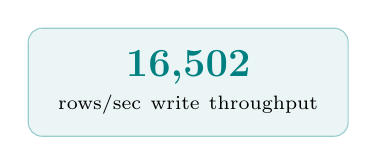
\begin{tikzpicture}
        \node[fill=DeepTeal!8,draw=DeepTeal!40,rounded corners=5pt,inner sep=8pt,text width=3.5cm,align=center] {%
          {\Large\bfseries\color{DeepTeal}16,502}\\{\scriptsize rows/sec write throughput}};
      \end{tikzpicture}
    \column{0.32\textwidth}
      \centering
      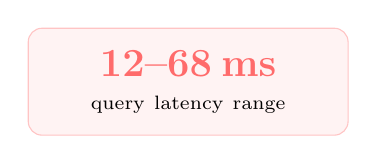
\begin{tikzpicture}
        \node[fill=Coral!8,draw=Coral!40,rounded corners=5pt,inner sep=8pt,text width=3.5cm,align=center] {%
          {\Large\bfseries\color{Coral}12--68 ms}\\{\scriptsize query latency range}};
      \end{tikzpicture}
    \column{0.32\textwidth}
      \centering
      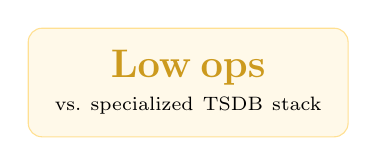
\begin{tikzpicture}
        \node[fill=Gold!10,draw=Gold!50,rounded corners=5pt,inner sep=8pt,text width=3.5cm,align=center] {%
          {\Large\bfseries\color{Gold!80!black}Low ops}\\{\scriptsize vs.\ specialized TSDB stack}};
      \end{tikzpicture}
  \end{columns}
\end{frame}
% ==================== SLIDE 12: LIVE DEMO ====================
\begin{frame}{Live Demo Plan}
  \begin{columns}[T]
    \column{0.32\textwidth}
      \centering
      
\begin{tikzpicture}
        \node[fill=DeepTeal!8,draw=DeepTeal!40,rounded corners=6pt,inner sep=10pt,text width=3.5cm,align=center,minimum height=3.2cm] {%
          {\fontsize{24}{24}\selectfont\textcolor{DeepTeal}{\faIcon{play-circle}}}\\[6pt]
          {\bfseries\color{DeepTeal}Demo }\\[4pt]
          {\small Watch Video}\\[6pt]
          {\scriptsize }};
      \end{tikzpicture}

  \end{columns}

  \vspace{0.5em}

\end{frame}


% ==================== SLIDE 14: IMPACT ====================
\begin{frame}{Impact and Scalability Path}
  \begin{columns}[T]
    \column{0.48\textwidth}
      \card{\faIcon{chart-line}\; Current Value}{%
        \begin{itemize}
          \item Real-time energy visibility
          \item Per-node and per-app analysis
          \item Early detection of unhealthy nodes
          \item Historical views for optimization
        \end{itemize}}
    \column{0.48\textwidth}
      \card{\faIcon{road}\; Scalability Path}{%
        \begin{itemize}
          \item \textbf{Today}: proof of concept on a small node set
          \item \textbf{Next}: tens to hundreds of nodes, same API
          \item \textbf{Later}: ClickHouse sharding + replicated backends
          \item No architecture redesign required
        \end{itemize}}
  \end{columns}

  \vspace{0.5em}
  \callout{We built a production-style distributed monitoring architecture based on autonomy, eventual consistency, adaptive health checking, and analytical storage.}
\end{frame}


% ==================== SLIDE 16: THANK YOU ====================
\begin{frame}[plain]
  \begin{tikzpicture}[remember picture,overlay]
    \fill[left color=DarkBg,right color=DarkBg!85!DeepTeal] (current page.south west) rectangle (current page.north east);
    % Decorative circles
    \fill[LightTeal,opacity=0.05] ([shift={(2.5cm,2.5cm)}]current page.south west) circle (2cm);
    \fill[LightTeal,opacity=0.04] ([shift={(-2cm,2cm)}]current page.south east) circle (2.5cm);
    \fill[LightTeal,opacity=0.06] ([shift={(-3cm,-2cm)}]current page.north east) circle (1.5cm);
    % Decorative rule
    \fill[LightTeal,opacity=0.6]
      ([shift={(-3cm,0.6cm)}]current page.center) rectangle ([shift={(3cm,0.64cm)}]current page.center);
    % Content
    \node at ([yshift=1.5cm]current page.center) {%
      {\fontsize{32}{38}\selectfont\bfseries\color{white}Thank You}};
    \node at ([yshift=-0.2cm]current page.center) {%
      {\Large\color{LightTeal}Questions?}};
    % Decorative rule
    \fill[LightTeal,opacity=0.6]
      ([shift={(-3cm,-0.7cm)}]current page.center) rectangle ([shift={(3cm,-0.66cm)}]current page.center);
    \node at ([yshift=-1.5cm]current page.center) {%
      {\small\color{MidGray}Distributed Energy Monitoring Platform}};
    % Accent bar at bottom (matching title slide)
    \fill[Coral] ([yshift=0.7cm]current page.south west) rectangle ([yshift=0.76cm]current page.south east);
    \fill[Gold,opacity=0.7] ([yshift=0.62cm]current page.south west) rectangle ([yshift=0.68cm]current page.south east);
    % Faded icons for visual interest
    \node[font=\fontsize{36}{36}\selectfont,text=DeepTeal,opacity=0.15]
      at ([shift={(5.5cm,1.5cm)}]current page.center) {\faIcon{bolt}};
    \node[font=\fontsize{28}{28}\selectfont,text=Coral,opacity=0.12]
      at ([shift={(-5.5cm,1cm)}]current page.center) {\faIcon{server}};
  \end{tikzpicture}
\end{frame}

\end{document}
